\chapter{How to Build a Fictional World --- Kate Messner}

Messner begins by doing something methodologically right. She does not start with a definition of worldbuilding. She starts with worlds that already work. Gandalf can die and return. In the Matrix, skill can be downloaded. A Cheshire Cat can juggle its own head. A Quidditch match does not end until the Golden Snitch is caught. The answer to the ultimate question is \(42\). Only after this parade of remembered laws does she tell us what holds them together: a fictional world is memorable not because it permits anything whatever, but because what it permits is governed by stable rules. The lecture then unfolds in a clean sequence: examples, principle, contrast with ordinary reality, the reader's grasp of the book-world, the deeper puzzle of how marks on a page become lived experience, and finally the practical method by which a writer builds a world and lets story emerge from it.

\section{Examples First: Worlds with Rules}

The lecture's opening is cumulative. Each example is a reminder that the strange becomes persuasive only when it is regular. Gandalf's body is mortal and his spirit immortal. The Matrix has a mechanism for accelerated competence. Cheshire Cat logic is absurd, but not formless. Quidditch has an explicit terminal condition. Even Douglas Adams's \(42\) has force because it sounds like the lawful output of a world whose questions and answers do not obey our own.

A compact note-form record of the opening is
\begin{align}
\text{mortal body} + \text{immortal spirit} &\Rightarrow \text{Gandalf can die and return},\\
\text{link up} + \text{hack code} &\Rightarrow \text{learn helicopter flight in seconds},\\
\text{Snitch caught} &\iff \text{Quidditch match ends},\\
\text{ultimate answer} &= 42.
\end{align}
These are not equations in the strict mathematical sense. They are local rule-statements. But Messner's point is that readers remember worlds through such rules. The marvel is legible because it has a form.

That lets the lecture make its first explicit abstraction:
\begin{equation}
\text{consistent rules} \Rightarrow \text{believability} + \text{comprehensibility} + \text{explorability}.
\end{equation}
A merely surprising world is thin. A world becomes explorable when one event teaches us how to read the next. The lecture therefore begins with examples not to entertain us before the real argument, but to make the real argument visible.

\subsection{Question \& Answer}

\paragraph{Question.} What makes an invented world feel coherent rather than random?

\paragraph{Answer.} Its wonders are constrained. Once the reader can infer what the world allows, forbids, or repeats, the world ceases to be a pile of novelties and becomes a domain with structure.

\section{Real Laws, Page Laws, and What Authors Actually Build}

From there Messner makes a sharper comparison. Gravity holds the Harry Potter books to their shelves in our world. We know this to be true. But on the pages of the fiction, once the wizarding domain has been established, gravity can be modified, suspended, or answered by another rule. The decisive distinction is not between law and lawlessness. It is between one lawful domain and another.

A useful compression of Messner's phrase ``a spectrum of physical and societal rules'' is the following.

\begin{definition}
We may summarize a fictional world schematically as
\begin{equation}
W = (R_{\mathrm{phys}},\,R_{\mathrm{soc}}),
\end{equation}
where \(W\) is the world, \(R_{\mathrm{phys}}\) its physical rules, and \(R_{\mathrm{soc}}\) its social rules. This is note-writer's notation, not notation from the lecture, but it captures the lecture's actual structure.
\end{definition}

The gravity contrast can then be written, cautiously, as
\begin{equation}
g_{\text{real world}} \neq g_{\text{wizarding page-world}}.
\end{equation}
The point of the shorthand is not to pretend that Messner is doing physics. The point is to make precise what her prose is already doing: distinguishing the law of the reader's world from the law of the world inside the book.

That is why she can immediately enlarge the scale. Authors of science fiction and fantasy do not merely choose a backdrop. They build a whole infrastructure of intelligibility:
\begin{equation}
\text{rules} \to \text{maps} \to \text{lineages} \to \text{languages} \to \text{cultures} \to \text{universes}.
\end{equation}
The arrows mark an increase in articulated structure. A single altered law gives us a trick. A connected system of laws, histories, and institutions gives us a world. At this point the lecture is ready to ask not only what worlds are, but what they do to readers.

\section{When the Reader Understands the Book-World}

Messner's next claim is the lecture's first major payoff. When worldbuilding is done well, the reader can understand the fictional world and its rules as well as the characters do, and sometimes even better than the reader understands the world outside the book. This is not a side remark. It is the proposition that creates the lecture's central tension. If that can happen, then we must ask how.

As a compact note-form comparison, we may write
\begin{equation}
\text{reader's grasp of book-world} \gtrsim \text{reader's grasp of outside world}.
\end{equation}
The symbol \(\gtrsim\) is only a shorthand for Messner's phrase ``just as well or even better.'' It is not spoken lecture notation. But it keeps the strength of the claim in view.

The one validated image from the lecture is useful precisely here. It is not an equation. It is a spatial contrast. The reader and open book occupy the foreground; a small story-world rises out of the pages; the outside world appears behind as a separate social field. The image shows what the sentence means: the world in the book can become, for a while, the more readable domain.

\begin{figure}[h]
\centering

\includegraphics[width=0.82\textwidth]{lecture_09_figure_03.png}
\caption{Reader, book-world, and the world outside the book.}
\end{figure}

Because the screenshot is rhetorical rather than symbolic, it helps to place a cleaned schematic beside it. We keep the screenshot as evidence and the TikZ redraw as interpretation.

\begin{figure}[h]
\centering
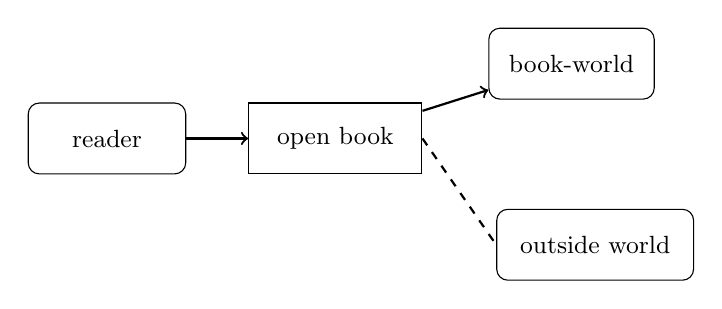
\begin{tikzpicture}[x=1cm,y=1cm]
\node[draw, rounded corners, minimum width=2.0cm, minimum height=0.9cm] (reader) at (0,0) {\small reader};
\node[draw, minimum width=2.2cm, minimum height=0.9cm] (book) at (2.9,0) {\small open book};
\node[draw, rounded corners, minimum width=2.1cm, minimum height=0.9cm] (inside) at (5.9,0.95) {\small book-world};
\node[draw, rounded corners, minimum width=2.5cm, minimum height=0.9cm] (outside) at (6.2,-1.35) {\small outside world};
\draw[->, thick] (reader) -- (book);
\draw[->, thick] (book) -- (inside);
\draw[dashed, thick] (book.east) -- (outside.west);
\end{tikzpicture}
\caption{A schematic reconstruction of the lecture's contrast between the world in the book and the world outside it.}
\end{figure}

The important thing is not the exact geometry of the redraw. It is the lecture's intuition: reading can produce a domain whose rules are more available to us than those of ordinary life.

\subsection{Question \& Answer}

\paragraph{Question.} How can a book-world become more legible than reality?

\paragraph{Answer.} Because the book-world is structured for intelligibility. Its rules are chosen, repeated, and made mutually supporting. Reality is richer, but also noisier. The lecture's point is that a well-built fictional world can therefore become, for the reader, the more tractable system.

\section{But How? How Squiggles Become Worlds}

At exactly this point Messner stops the forward movement and asks the lecture's largest question: but how? How can squiggles on a page reflect light into the eye, send signals to the brain, be decoded as narrative, move us emotionally, and finally alter the way we return to the world after the last mark has been read?

The lecture's own chain may be written compactly as
\begin{equation}
\text{squiggles on page} \to \text{signals to the brain} \to \text{decoded narrative} \to \text{emotion/thought/action} \to \text{changed perspective}.
\end{equation}
Here we should preserve the lecture's rhythm. Messner does not reduce the matter to information transfer alone. She explicitly widens the chain from perception to feeling, from feeling to action, and from action to altered perspective. The end of reading is not mere comprehension. It is transformation, however small.

\paragraph{Worked derivation.} Unpacked into steps, the lecture's mechanism becomes
\begin{enumerate}
\item Marks are placed on the page.
\item Light reflected from the page reaches the eyes.
\item The nervous system converts that input into signals.
\item The mind decodes patterned signals as narrative.
\item Narrative recruits emotion, thought, and imagination.
\item The reader enters the fictional world as a lived domain.
\item On leaving the book, the reader's view of the ordinary world may be different.
\end{enumerate}

This is a functional derivation, not a finished science of reading. Messner is careful about that. She explicitly says she is not sure anyone fully knows the answer. That concession matters. The lecture does not pretend to solve the mystery in order to get on with craft. It lets the mystery stand, and then turns toward practice anyway.

\subsection{Question \& Answer}

\paragraph{Question.} How do marks on a page become a lived world in the reader's mind?

\paragraph{Answer.} The lecture answers by chain rather than by theorem. Marks become signals, signals become decoded order, decoded order becomes narrative, and narrative recruits feeling strongly enough to produce immersion and return. The exact mechanism remains partly obscure; the operative sequence is plain.

\section{From Mystery to Method}

Once the lecture has allowed the mystery to stand, it changes scale. Fantastical worlds, Messner says, are created every day: in our minds, on computers, even on napkins. The practical premise is that imagination, together with the willingness to live inside imagination, is enough to begin. The lecture then descends into a writer's method.

The first step is historical:
\begin{equation}
\text{past events} \to \text{timeline} \to \text{present structure of the world}.
\end{equation}
This is a stronger claim than it first appears to be. We do not begin with decoration. We begin by asking what happened, in what order, and with what long consequences. A timeline is therefore not extra material; it is the first formal answer to the question of why the world is arranged as it is.

From there Messner proceeds by ordered families of questions. At the macro scale we ask about law, power, belief, and value:
\begin{equation}
(\text{rules},\ \text{government},\ \text{power},\ \text{beliefs},\ \text{values}).
\end{equation}
At the scale of ordinary life we descend into lived texture:
\begin{equation}
(\text{weather},\ \text{home/work/school},\ \text{food},\ \text{play},\ \text{young/old},\ \text{plants/animals},\ \text{technology},\ \text{transportation},\ \text{communication},\ \text{information}).
\end{equation}
The ordering is pedagogically exact. We move from constitutive law to social structure, and only then to daily life. A world is not yet inhabitable when we know its slogans. It becomes inhabitable when we know what people eat, how they move, what they fear, what they teach, what they punish, and what sort of weather meets them in the morning.

\paragraph{Worked example.} Messner's method can be rewritten as a disciplined update rule for the world-description.
\begin{enumerate}
\item Specify the world's past and organize it as a timeline.
\item Determine which physical and social rules are in force.
\item Ask who governs, who has power, and what people believe.
\item Ask what the society values and how it handles violation.
\item Descend into daily realities: weather, work, school, food, play, age, ecology, and technology.
\item Continue until the world ceases to be a list and becomes a place.
\end{enumerate}
The lecture is not asking for exhaustive paperwork. It is asking for enough structured attention that the world begins to answer back coherently.

\section{From World to Story}

Only at the end does Messner reveal the lecture's real destination. Worldbuilding is not the endpoint. Story is. Once we know the world as well as we hope the reader will know it, we set characters free inside it and ask what follows. The world then stops being background and becomes causal.

Messner's closing compression is
\begin{equation}
\text{world} + \text{characters} \Rightarrow \text{shaped individuals} \Rightarrow \text{conflict} \Rightarrow \text{story}.
\end{equation}
This equation deserves to stand at the end because it reinterprets everything that came before. The rules were never only ornamental. The timeline was never only archival. The questionnaire was never only descriptive. All of it was preparation for pressure. A world shapes what its inhabitants can want, what they can fear, what they can violate, what they can become, and therefore what kinds of conflict can appear.

We can put the point more bluntly. A world without people gives us a dossier. People without a world give us abstractions. Story begins when structured people meet a structured world and are forced to move under its constraints.

\subsection{Question \& Answer}

\paragraph{Question.} When does worldbuilding stop being background and start becoming story?

\paragraph{Answer.} It becomes story when the world's structure begins to govern choice. Once characters must live under the world's rules, values, technologies, punishments, and permissions, conflict appears. At that point the world is not scenery. It is one of the active terms in the drama.

\section{Summary}

Messner's lecture gives us a compact but genuine mathematics of fictional worlds. Strong invented worlds are rule-governed. Their laws may differ sharply from those of ordinary life, but the difference must itself be coherent. When the construction succeeds, readers can learn the internal world of the book with extraordinary clarity. That fact raises the deeper puzzle of how marks on a page become lived experience, and the lecture lets that puzzle remain partly mysterious. But it then gives us a practical answer at the level of craft: construct the world's past, specify its laws and institutions, descend into daily life, and then let characters move inside the resulting structure. At that moment, worldbuilding stops being preparation and becomes story.